\fontsize{9.5pt}{7.2}\selectfont

\section{Dominio abierto (Qanus/Freeling/CLEF)}

%%%%%%%%%%%%%%%%%%%%%%%%%%%%%%%%%%%
%%
%%			Introducción
%%
%%%%%%%%%%%%%%%%%%%%%%%%%%%%%%%%%%%
\subsection{Introducción}

\begin{frame}[<+->]
\frametitle{Introducción}
  \begin{itemize}
    \item Sistema QA de dominio abierto con soporte multilingüe
    \item Basado en Qanus, adaptado para usar Freeling.
    \begin{itemize}
      \item Pipeline - IR + NLP + Heurísticas
    \end{itemize}
    \item Ejercicios de CLEF'07 monolingüe para español (es-es) y portugués (pt-pt)
    \begin{itemize}
      \item Wikipedia como base de conocimiento (\st{newsletters})
      \item Factoids (\st{lists}, \st{definition})
      \item Respuesta exacta. Nulas. Tópicos por grupo con co-referencia.
    \end{itemize}
    \item Agregamos: 
    \begin{itemize}
        \item Heurísticas de generación de queries (de Lasso y de \textit{topics})
        \item Heurística de ranking de pasajes
    \end{itemize}
    \item Experimentamos y sacamos conclusiones.
  \end{itemize}


\end{frame}



\begin{frame}
\frametitle{Preguntas}
  \begin{center}
  \begin{table}
  \centering
  \begin{tabular}{| l | l | l | l | l | l |}
  
  Subset & Idioma & Factoid & Definition & List & Total \\ 
  \multirow{2}{*}{Todo} & es & 158 & 32 & 10 & 200 \\ 
   & pt & 159 & 31 & 10 & 200 \\ \hline
   \multirow{2}{*}{Wiki} & es & \textbf{122} & 24 & 9 & 163 \\ 
   & pt & \textbf{104} & 18 & 8 & 130 \\ 
  \end{tabular}
  \caption{Totales por tipo de pregunta}
  \label{table:totals-type-question}
  \end{table}
  \end{center}

  Ejemplo de grupo con tema y correferencia (primer cluster de preguntas para es-es):
  \begin{itemize}
  \item ¿En qué colegio estudia Harry Potter?
  \item ¿Cuál es el lema del colegio?
  \item ¿En qué casas está dividido?
  \item ¿Quién es el director del colegio?
  \end{itemize}

\end{frame}


%%%%%%%%%%%%%%%%%%%%%%%%%%%%%%%%%%%
%%
%%			Marco teórico
%%
%%%%%%%%%%%%%%%%%%%%%%%%%%%%%%%%%%%
\subsection{Marco teórico}


\begin{frame}
\frametitle{Marco teórico / arquitectura de pipeline}
  \begin{figure}
      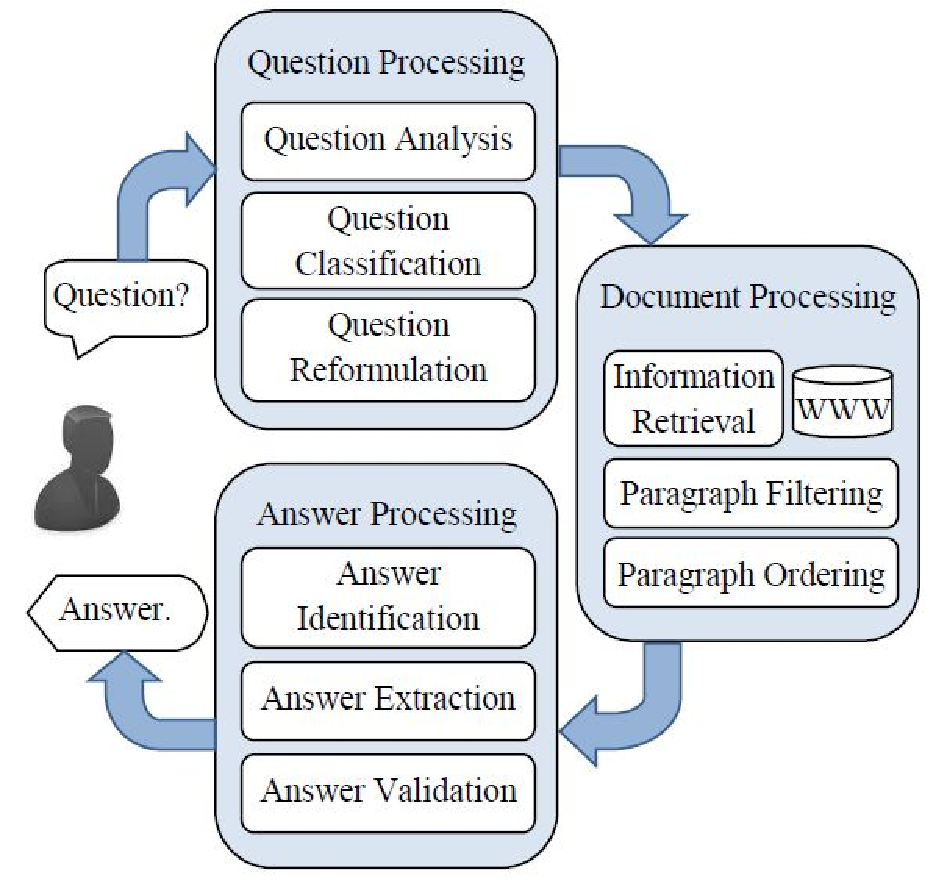
\includegraphics[scale=0.4]{graficos/qa-open-domain}
    \caption{Módulos y submódulos de un sistema de QA (ver prox slide)}
    \label{fig:tareas}
  \end{figure}
\end{frame}


\fontsize{8.5pt}{7.2}\selectfont
\begin{frame}[<+->]
\frametitle{Marco teórico / arquitectura de pipeline}
  \begin{block}{Módulo de procesamiento de la pregunta}
    \begin{itemize}
      \item Submódulo principal: Question Classifier. Question Type
      \item Anotaciones de la pregunta (NER, POS)
      \item Creación de consulta para IR (Heurística de Lampert, Moldovan)
    \end{itemize}
  \end{block}
  \begin{alertblock}{Módulo de procesamiento de documentos}
    \begin{itemize}
      \item Submódulo principal: índice invertido (estructuras de IR)
      \item División en parágrafos
      \item Filtrado grueso
      \item Re-ranking de parágrafos
    \end{itemize}
  \end{alertblock}
  
  \begin{exampleblock}{Módulo de procesamiento de la respuesta}
    \begin{itemize}
      \item Heurísticas específicas basadas en casos.
      \item Identificación de respuestas candidatas y re rankeo
      \item Extracción de respuestas
    \end{itemize}
  \end{exampleblock}
\end{frame}


\begin{frame}
\frametitle{Indice Invertido}
  \begin{figure}
      \includegraphics[scale=0.6]{graficos/presentacion/i-i}
    \caption{Indice invertido}
    \label{fig:tareas}
  \end{figure}
\end{frame}



\begin{frame}\fontsize{7.5pt}{7.8}\selectfont
  \frametitle{POS - part-of-speech tagging - etiquetado gramatical}

\begin{center}
\begin{tabular}{| l | l |}
 \hline
Categoría Gramatical & Ejemplos \\ \hline
Determinante & aquel, este, mi, sus, nuestras \\ \hline
Pronombre & yo, tú, él, mí, nos, aquéllos, suyos \\ \hline
Preposición & a, ante, bajo, con, contra\\ \hline
Conjunción & y, aunque, pero, incluso\\ \hline
Interjección & ah, eh, ejem\\ \hline
\textbf{Sustantivo} & chicos, tesis, Pedro, cortapapeles\\ \hline
\textbf{Verbo} & cantamos, corrió, bailarán\\ \hline
\textbf{Adjetivo} & alegre, bonita, pésimos, desnuda\\ \hline
Adverbio & despacio, hábilmente, posteriormente\\ \hline
\end{tabular}
\end{center}

  \begin{alertblock}{POS - \dq{El hombre bajó la escalera.}}
  \begin{table}
    \begin{tabular}{| l | l | l |}
    \hline
    Forma &  Etiqueta & Descripción \\ \hline
    El & DA0MS0 & Determinante, Artículo, Masculino, Singular\\
    hombre & NCMS000 & Nombre, Común, Masculino, Singular  \\ 
    bajó & VMIS3S0 & Verbo, Principal, Indicativo, Pasado, Tercera Persona, Singular\\ 
    la & DA0FS0 & Determinante, Artículo, Femenino, Singular\\ 
    escalera& NCFS000 & Nombre, Común, Femenino, Singular \\ 
    .& Fp& Punto final\\ \hline
  \end{tabular}
  \end{table}
  \end{alertblock}

\end{frame}

\fontsize{9.5pt}{9.2}\selectfont

\begin{frame}
  \frametitle{NER - Named entities recognition - Reconocimiento de Entidades Nombradas}
  Reconoce: Personas, Organizaciones, Lugares. \newline

  Lionel Messi nació el 24 de junio de 1987 en la ciudad de Rosario, en la provincia de Santa Fe. Es hijo de Jorge Horacio Messi, trabajador de una fábrica, y de Celia María Cuccittini, una limpiadora de medio tiempo (...).\newline

  Con apenas cinco años, Messi dio sus primeros pasos en Grandoli, un club de barrio al sur de Rosario, a pocas cuadras de su casa. El club estaba dirigido por su padre. Posteriormente jugó algunos partidos con el Central Córdoba. En 1995, comenzó a entrenarse en las divisiones inferiores de Newell's Old Boys.
\end{frame}


\begin{frame}
  \frametitle{NER - Named entities recognition - Reconocimiento de Entidades Nombradas}
  Reconoce: {\color{red}Personas}, {\color{blue}Organizaciones}, {\color{green}Lugares}. \newline

  {\color{red}Lionel Messi} nació el 24 de junio de 1987 en la ciudad de {\color{green}Rosario}, en la provincia de {\color{green}Santa Fe}. Es hijo de {\color{red}Jorge Horacio Messi}, trabajador de una fábrica, y de {\color{red}Celia María Cuccittini}, una limpiadora de medio tiempo (...).\newline

  Con apenas cinco años, {\color{red}Messi} dio sus primeros pasos en {\color{blue}Grandoli}, un club de barrio al sur de {\color{green}Rosario}, a pocas cuadras de su casa. El club estaba dirigido por su padre. Posteriormente jugó algunos partidos con el {\color{blue}Central Córdoba}. En 1995, comenzó a entrenarse en las divisiones inferiores de {\color{blue}Newell's Old Boys}.


\end{frame}

\begin{frame}
  \frametitle{QC - Clases de preguntas}
  \begin{figure}
      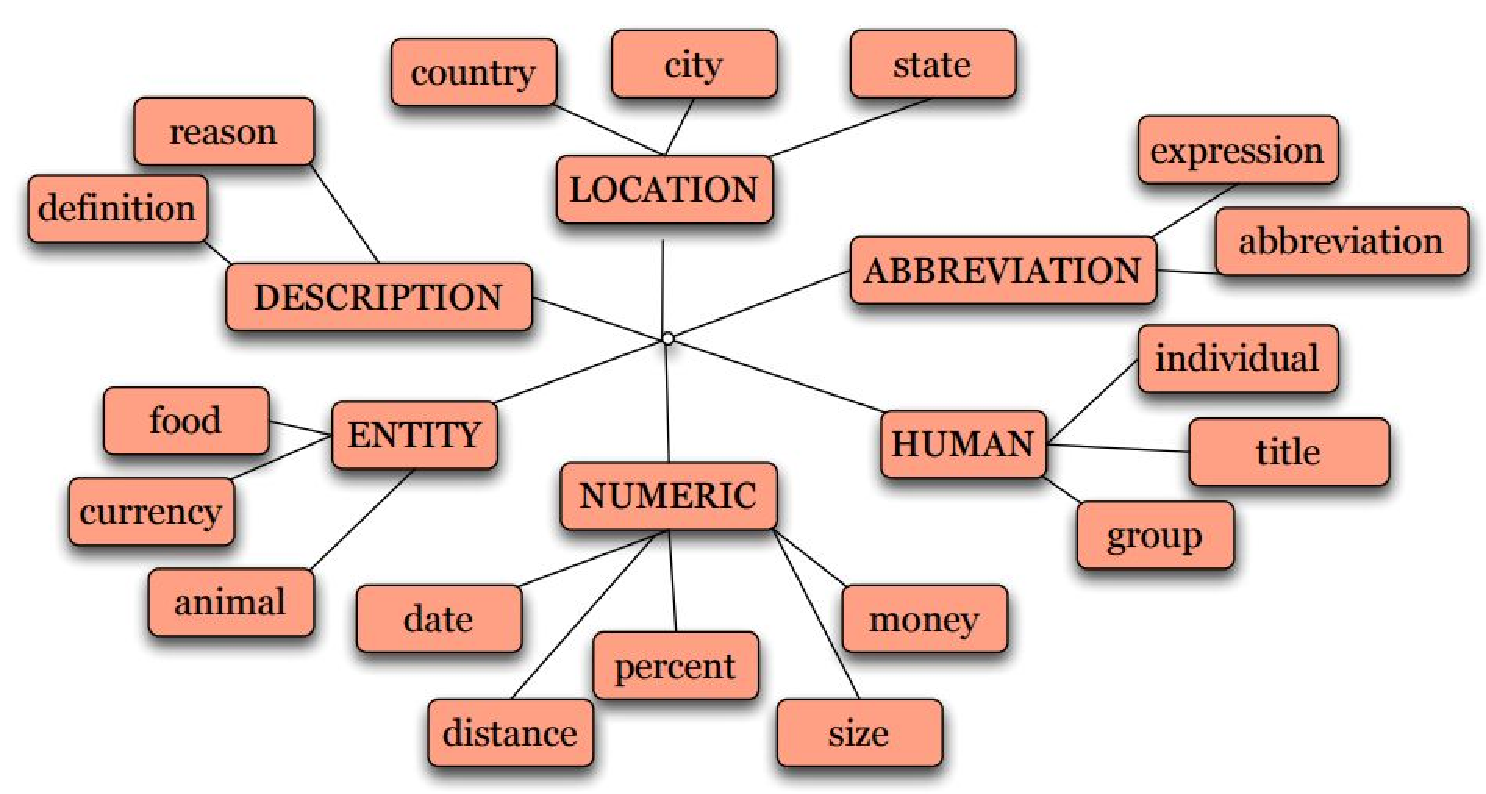
\includegraphics[scale=0.4]{graficos/li-roth-qc-classes}
    \caption{Clases de Question Type para el QC de Stanford}
    \label{fig:tareas}
  \end{figure}
\end{frame}



% \begin{frame}
% \frametitle{Heurística de generación de queries [Lampert, 2004]}
% \begin{block}{8 pasos}<1->
% \begin{enumerate}
% \item Palabras no stop words entre comillas
% \item Entidades nombradas reconocidas
% \item Construcciones nominales con sus adjetivos
% \item Demás construcciones nominales
% \item Sustantivos con sus adjetivos
% \item Demás sustantivos
% \item Verbos
% \item El \sq{focus} de la pregunta
% \end{enumerate}
% \end{block}
% \end{frame}

%%%%%%%%%%%%%%%%%%%%%%%%%%%%%%%%%%%
%%
%%			Implementación
%%
%%%%%%%%%%%%%%%%%%%%%%%%%%%%%%%%%%%
\subsection{Implementación}

%%%%%%%%%%%%%%%%%%%%%%%%%%%%%%%%%%%
%%
%%      Ejercicio de Clef
%%
%%%%%%%%%%%%%%%%%%%%%%%%%%%%%%%%%%%


% \begin{frame}
%   \frametitle{Tareas activadas en Clef '07}
%   \begin{figure}
%       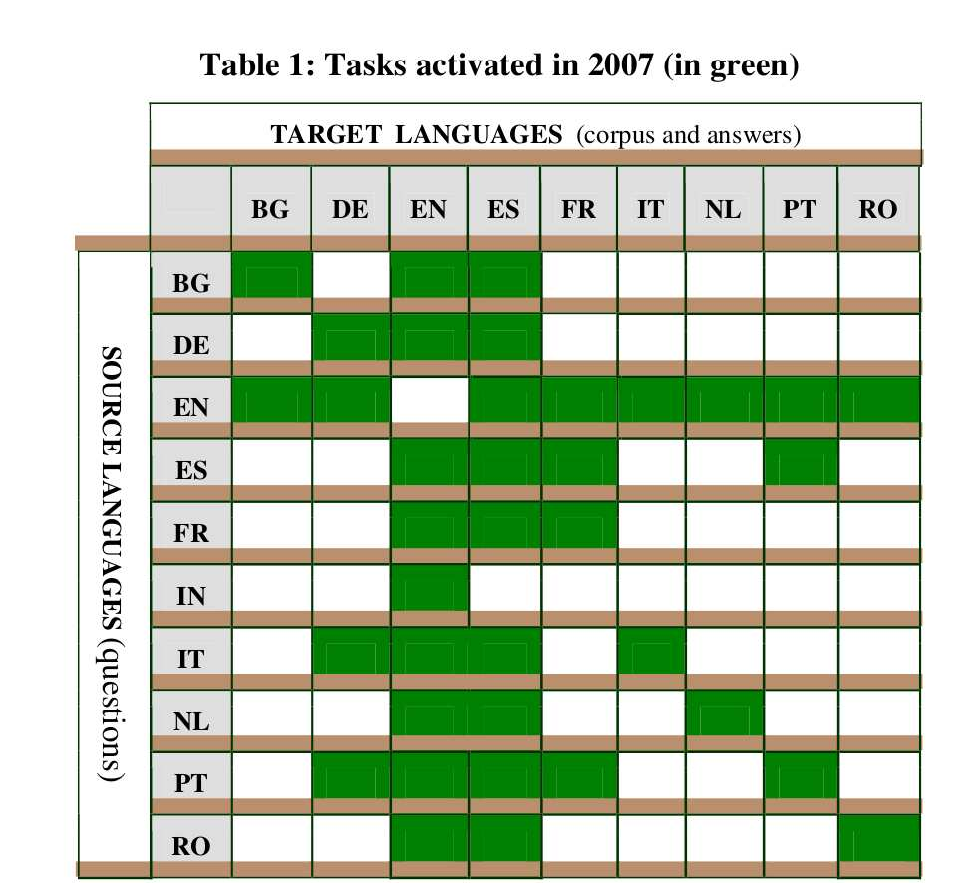
\includegraphics[scale=0.4]{graficos/clef07}
%     \caption{Tareas activadas en la competencia Clef '07}
%     \label{fig:tareas}
%   \end{figure}
% \end{frame}


%%%%%%%%%%%%%%%%%%%%%%%%%%%%%%%%%%%
%%
%%      Sistema
%%
%%%%%%%%%%%%%%%%%%%%%%%%%%%%%%%%%%%
\subsubsection*{Sistema}

\begin{frame}[<+->]
\frametitle{Qanus}
  \begin{alertblock}{\textit{Question-Answering @ National University of Singapore}}
  \begin{itemize}
    \item Un framework de question answering basado en information retrieval
    \item QA-sys: un sistema de QA funcional simple construido sobre este framework. 
    %\item Actualizado por última vez en noviembre de 2012, código abierto
    \item Herramientas de NLP de Stanford (POS, NER y QC, para inglés) y Lucene. 
    \item Estructura de Pipeline. Orientado para TREC 07 (Aquaint)
  \end{itemize}
  \end{alertblock}
\end{frame}

\begin{frame}
\frametitle{Qanus}
  \begin{figure}
      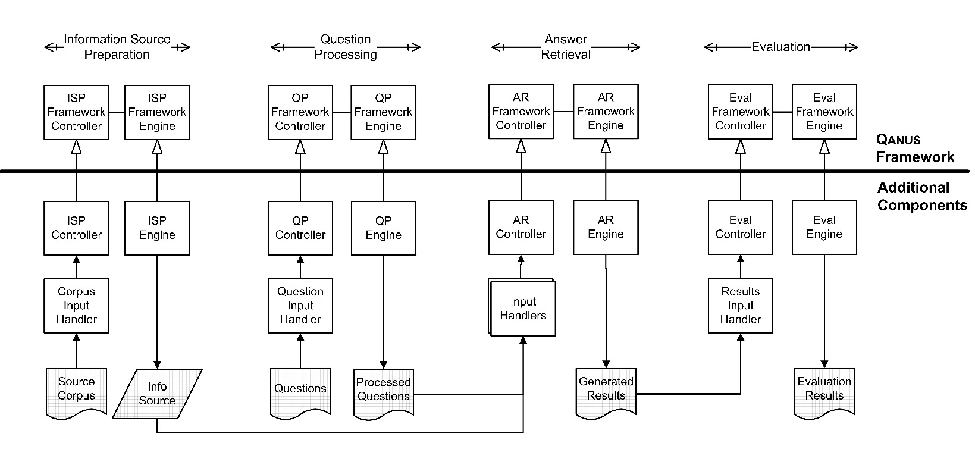
\includegraphics[scale=0.7]{graficos/Quanus}
    \caption{El framework Quanus y la implementación QA-sys}
    \label{fig:Quanus}
  \end{figure}
\end{frame}


\begin{frame}
\frametitle{QA-Sys - Qanus @ TREC 07}
\begin{columns}[T] % align columns
\begin{column}{.48\textwidth}
  \begin{figure}
      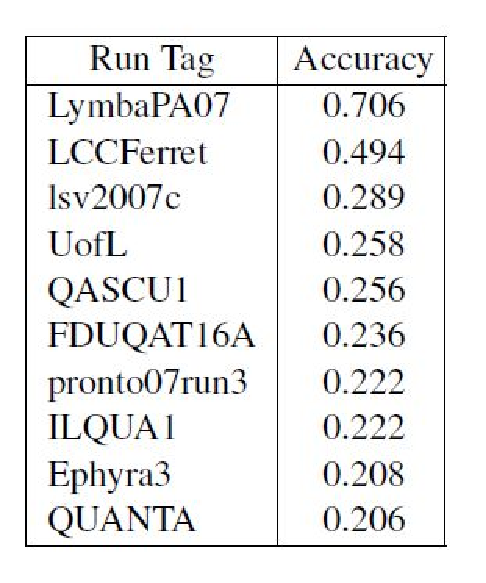
\includegraphics[scale=0.5]{graficos/trec-7-accuracy-reduced}
    \caption{Resultados de Trec 07}
    \label{fig:tareas}
  \end{figure}
\end{column}%
\hfill%
\begin{column}{.48\textwidth}

  \begin{block}{TREC 07}
      \begin{itemize}
          \item Monolingue, Inglés. %Competencia importante
          \item 200 preguntas
          \item Evaluada por humanos
          \item \textit{Precisión}: respuestas exactas sobre respuestas totales
          \item LymbaPA $\rightarrow$ {\color{blue}0.706} (70\%)
          \item QA-Sys $\rightarrow$ {\color{blue}0.119} (12\%)
        \end{itemize}
  \end{block}
\end{column}%
\end{columns}

\end{frame}


\begin{frame}
\frametitle{Baseline: QA-Sys}
  \textbf{1. Preparación de la fuente de información: } Preprocesa XML de Aquaint de manera offline en un índice Lucene. \newline

\textbf{2. Análisis de la pregunta: } \newline Anota la pregunta con POS, NER y QC. \newline

\textbf{3. Generación de respuestas: } Busca la pregunta en el índice, separa los documentos en pasajes y los rankea con métricas heurísticas y luego, dependiendo del tipo de QC, aplica heurísticas basadas en NER, POS y QC sobre los pasajes para extraer una respuesta.\newline

\medskip

\begin{exampleblock}{ML QA-Sys}
  \begin{itemize}
    \item Soporte multi idioma no simultaneo.
    \begin{itemize}
      \item Soporta varios idiomas, pero de a uno a la vez.
    \end{itemize}
    \item Indice invertido de Wikipedia
    \item Reemplazamos las herramientas NLP por Freeling y sacamos reglas dependiente al idioma.
  \end{itemize}
\end{exampleblock}

\end{frame}


\begin{frame}
\frametitle{Pipeline}
  \begin{figure}
      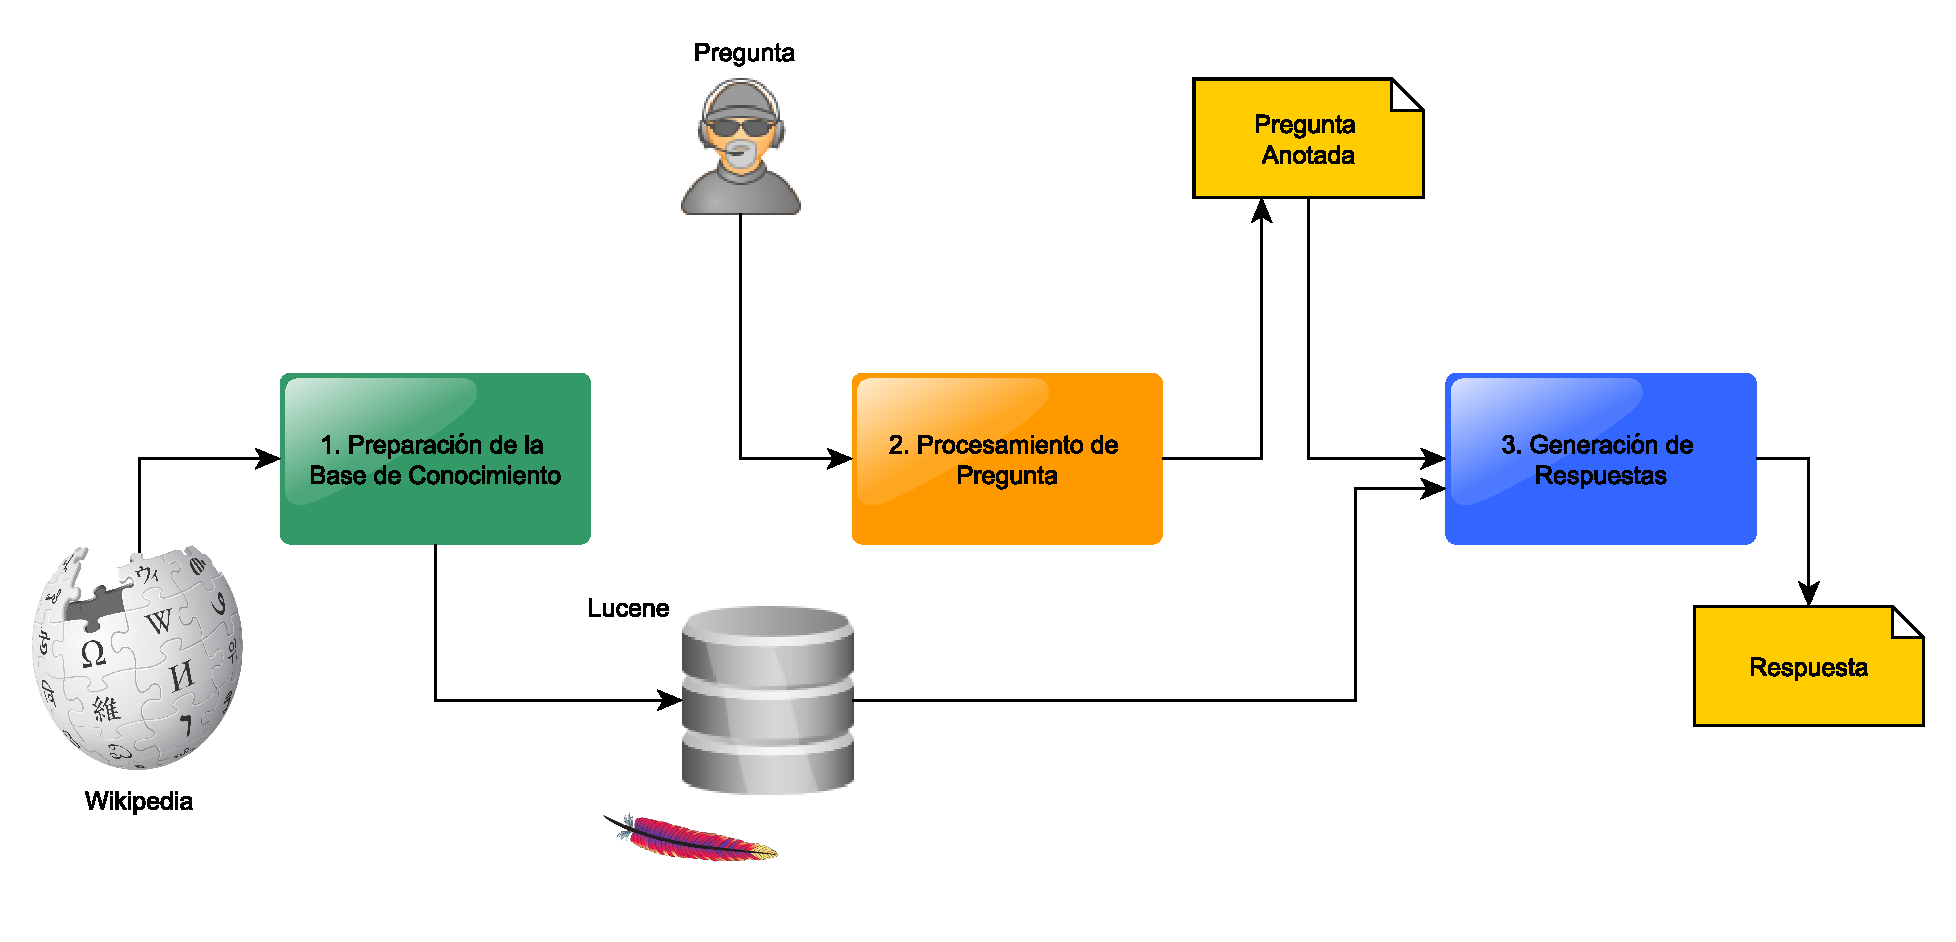
\includegraphics[scale=0.3]{graficos/pipeline}
  \end{figure}
\end{frame}


\begin{frame}
\frametitle{1. Preparación de la base de conocimiento}
  \begin{figure}
      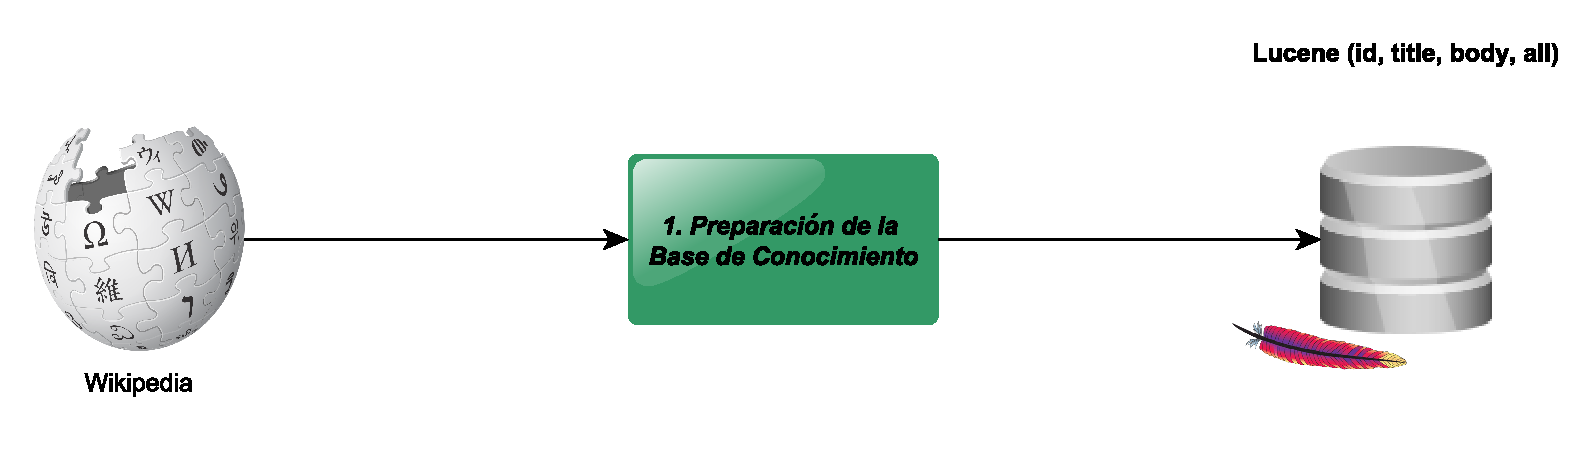
\includegraphics[scale=0.33]{graficos/pipeline-ibp}
  \end{figure}
    \begin{table}
    \centering
    \begin{center}
    \begin{tabular}{| l | l | l | l | l | l| l|}
    Wikipedia & \# Entradas & Nulas & Redirects & Filtradas & \textbf{Válidas} \\ 
    %simple-06 & 18273 & 22 &  3452 & 5241 & 9558 \\ 
    %simple-13 & 180067 & 8 & 35600 & 41902 & 102557\\
    \textbf{es-06} & \textbf{233750} & 52 & 62805 & 34947 & \textbf{{\color{green}135946}} \\ 
    \textbf{pt-07} & \textbf{498039} & 80 & 210983 & 43390 & \textbf{{\color{green}243586}} \\ 
    \end{tabular}
    \caption{Wikipedias: cantidad de entradas válidas e inválidas}
    \label{table:creacion-indices}
    \end{center}
    \end{table}
\end{frame}


% \begin{frame}
% \frametitle{2. Procesamiento de la pregunta}
%   \begin{figure}
%       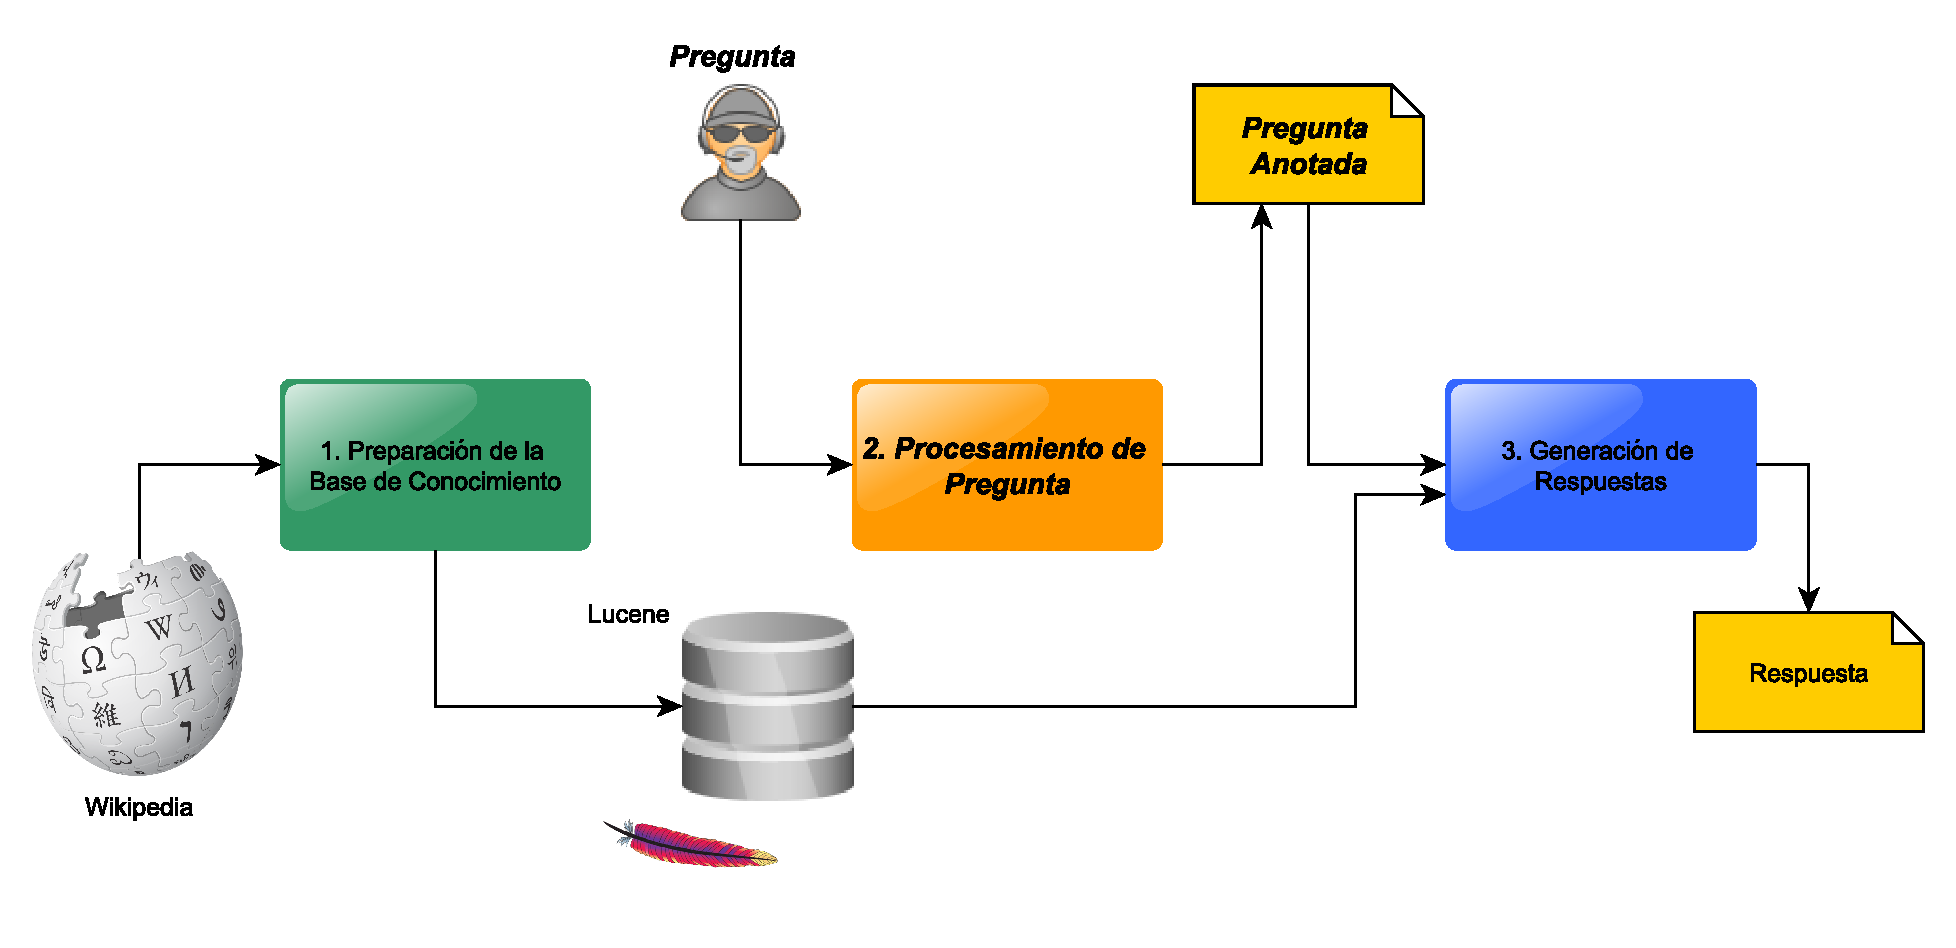
\includegraphics[scale=0.3]{graficos/pipeline-qp}
%     \label{fig:Quanus}
%   \end{figure}
% \end{frame}

\begin{frame}
\frametitle{2. Procesamiento de la pregunta}
  \begin{itemize}
    \item NER $\rightarrow$ Freeling
    \item POS $\rightarrow$ Freeling
    \item QC $\rightarrow$ No hay en ES ni PT
    \begin{itemize}
        \item Aprovechando que estaban activas las tareas en-es y en-pt
        \item Hack (truchada)  $\rightarrow$ pasamos QC sobre preguntas en inglés
    \end{itemize}
  \end{itemize}

  \begin{table}
    \centering
    \begin{center}
    \begin{tabular}{| l | l | l | }
    Clase & \# ES  & \# PT \\ 
    HUM &  62 & 53 \\ 
    NUM &  53 & 52\\ 
    ENTY &  34 & 28\\ 
    DESC &  25 & 30\\ 
    LOC &  24 & 36\\ 
    ABBR &  2 & 1\\ 
    Total & 200 & 200 \\
    \end{tabular}
    \caption{Clases de las preguntas para ES y PT, Stanford Classifier (Li \& Roth, Stanford)}
    \label{table:qc-es-pt}
    \end{center}
  \end{table}
\end{frame}




% \begin{frame}
% \frametitle{Pipeline}
%   \begin{figure}
%       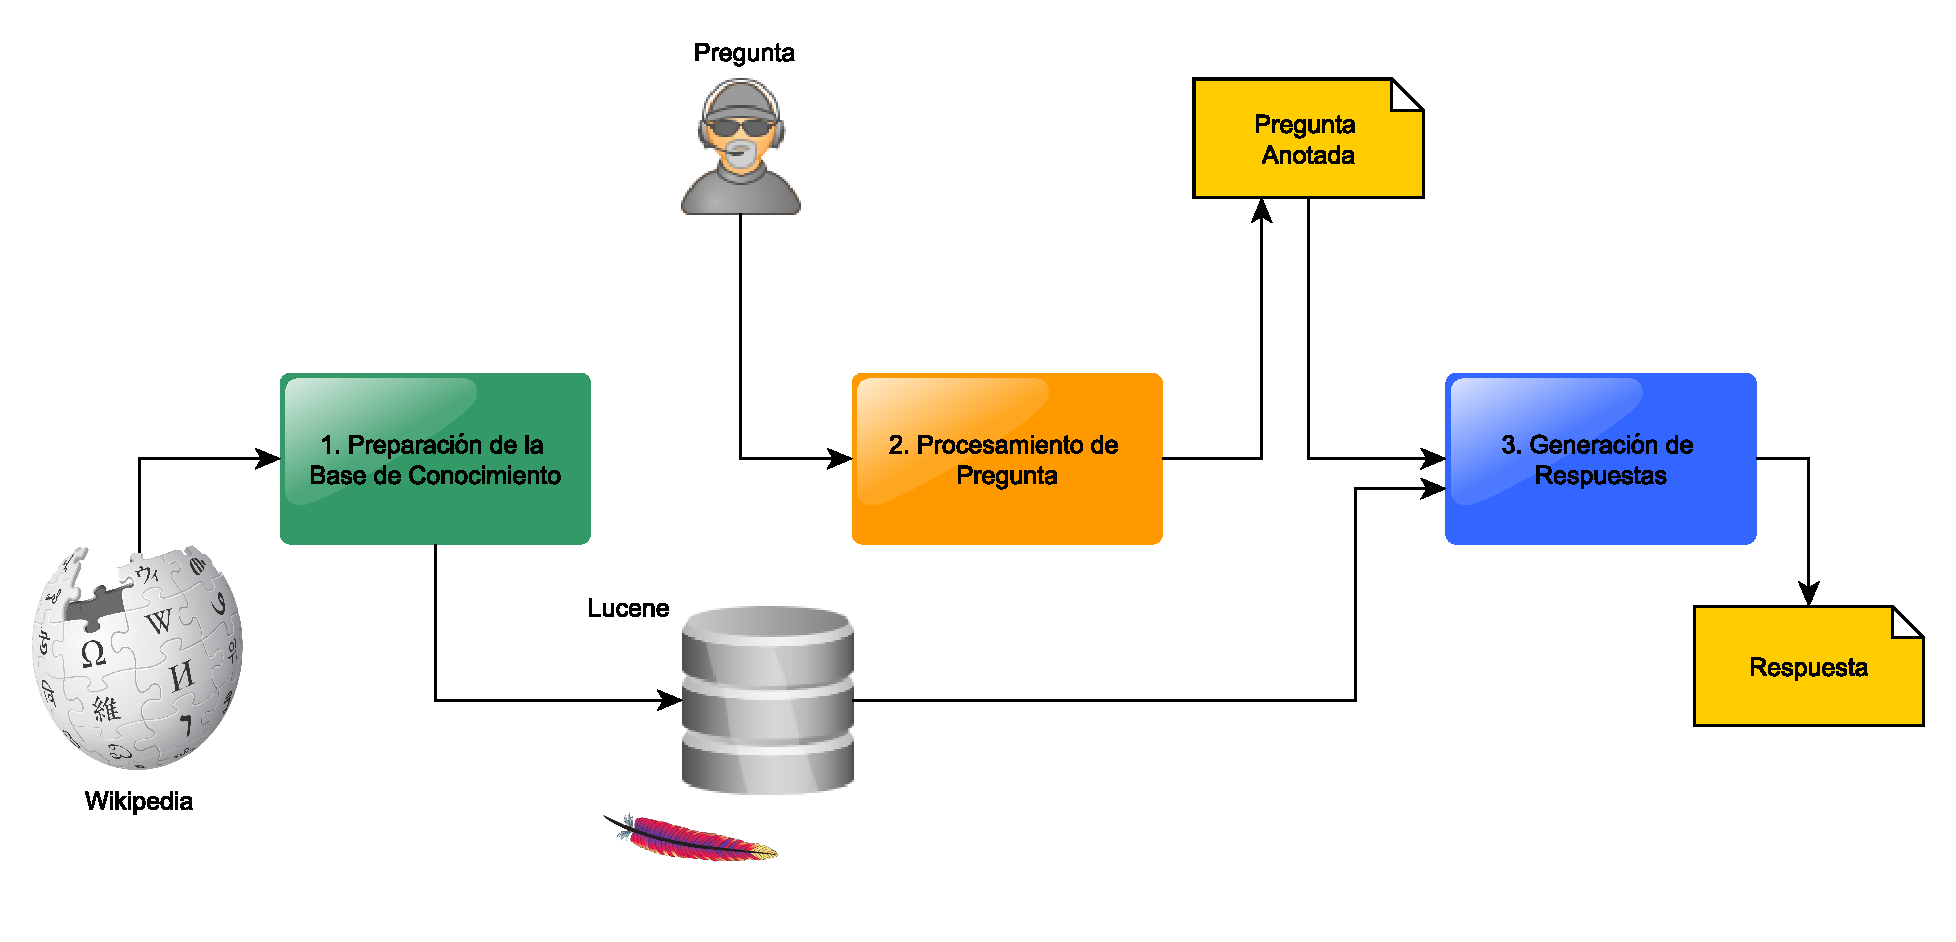
\includegraphics[scale=0.3]{graficos/pipeline}
%     \caption{Pipeline}
%     \label{fig:Quanus}
%   \end{figure}
% \end{frame}

\begin{frame}[<+->]
\frametitle{3. Generación de Respuestas}
  \begin{columns}[T] % align columns
\begin{column}{.38\textwidth}
      \begin{figure}
          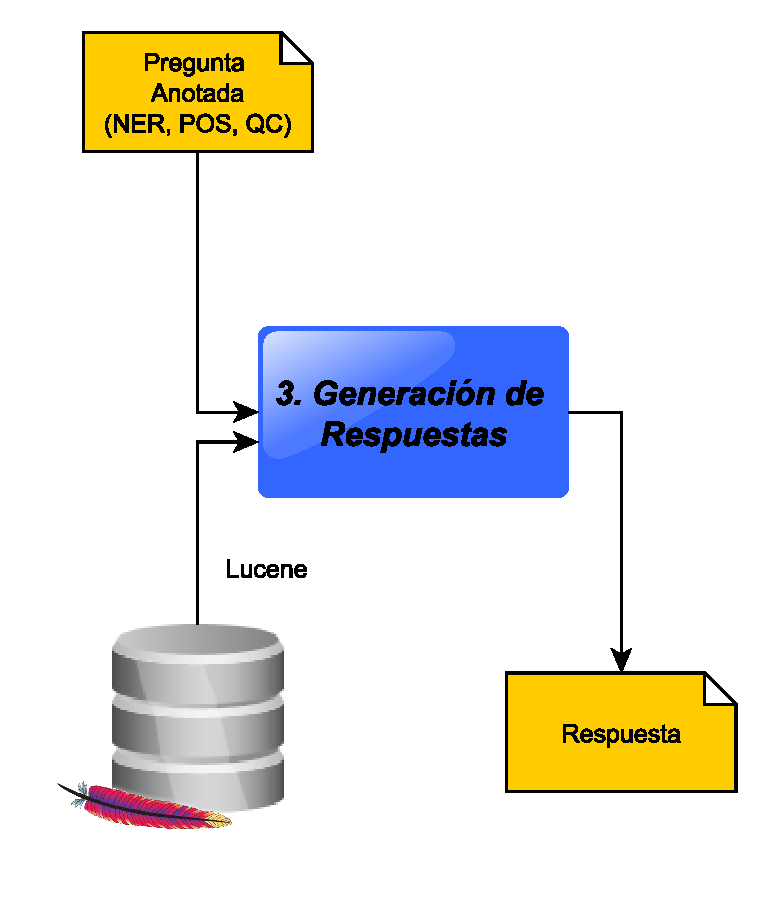
\includegraphics[scale=0.3]{graficos/pipeline-ar}
        %\caption{Módulos y submódulos de un sistema de QA}
        %\label{fig:tareas}
      \end{figure}
\end{column}%
\hfill%
\begin{column}{.58\textwidth}
El algoritmo tiene los siguientes pasos:
  \begin{enumerate}
    \item Generación de Queries
    \item Information Retrieval (documentos)
    \item Extracción y rankeo de oraciones
    \item POS tagging de las mejores oraciones
    \item Heurísticas de AR basadas en el QC
    \begin{itemize}
      \item \fontsize{8.5pt}{7.2}\selectfont Detectar respuestas candidatas
      \item \fontsize{8.5pt}{7.2}\selectfont Re rankearlas según lógica específica
      \item \fontsize{8.5pt}{7.2}\selectfont Extraer respuesta
    \end{itemize}
  \end{enumerate}
\end{column}%
\end{columns}
\end{frame}

\begin{frame}
\frametitle{3. Generación de Respuestas (2)}
  \begin{block}{Generación de Queries}
  \begin{itemize}
      %\item Descartamos caso (\dq{Who (is|was) (the) NN ... NN?} )
      \item Caso baseline
      \begin{itemize}
        \item Input: pregunta + \sq{target}(TREC) / tópico (CLEF)
        \begin{itemize}
              \item Palabras no stop-words de \textit{target} 
              \item Sustantivos, verbos y adjetivos de la pregunta.
        \end{itemize}
      \end{itemize}
      \item Evaluamos 3 métodos para generar queries
      \item Evaluamos 4 métodos para generar target
    \end{itemize}
  \end{block}

    \begin{exampleblock}{Extracción y re rankeo de oraciones post IR}
    \begin{itemize}
      \item Documentos divididos en oraciones
      \item Re rankeo de oraciones con \textit{scorers}:
      \item $rank = 0.9\times covr + 0.05\times freq + 0.05\times prox;$ %\footnotemark
      \item Primeras 40 oraciones pos-taggeadas, el resto se desecha
      \item Evaluamos 6 métodos para rankear
    \end{itemize}
  \end{exampleblock}
\end{frame}



\begin{frame}
\frametitle{Scorers: covr, freq, prox}
  \begin{block}{cov \& freq: Ocurrencia de la query en la respuesta candidata}
  \begin{itemize}
      \item Cubrimiento: $\frac{\text{tokens de la query que ocurren en la oración}}{\text{tokens de la query}}$
      \item Frecuencia: $\frac{\text{tokens de la query que ocurren en la oración}}{\text{tokens de la oración}}$
  \end{itemize}
  \end{block}
  \begin{alertblock}{Prox: distancia de dos strings en un tercero}
  \begin{itemize}
      \item $s_1=$\dq{Argentina es un país americano} y $s_2=$\dq{independizado en 1810}
      \item $t=$\dq{Argentina es un país americano, originalmente una colonia española, independizado en 1810}
      \item $prox(s_1, s_2, t)= \frac{dist(s_1, s_2)}{len(t)} = \frac{7}{12} = 0.58 $, 
      \begin{itemize}
          \item $dist(s_1, s_2)=$ cantidad de strings entre \sq{un} y \sq{en} (tokens intermedios de $s_{1,2}$)
          \item $len(t)=$ cantidad de strings del texto
          \item $~$1 denota que los dos string están cercanos uno al otro en el tercer string.
      \end{itemize}
  \end{itemize}
  \end{alertblock}
\end{frame}


  % \begin{frame}
  % \frametitle{Scorers: Span}
  %   \begin{block}{Span: similar a Prox, pero sobre un string y sus tokens}
  %   \begin{itemize}
  %   \item $s = \{token_1, token_2, ..., token_n\}$ y $t$ un texto
  %   \item Sea $r$ la cantidad de tokens de $s$ que aparecen en $t$
  %   \item Sea $d$ la distancia de los tokens de $s$ más distantes en $t$
  %   \item Entonces, $\text{Span}=fraq{r}{d}$
  %   \item Un score cercano a 1 significa que los términos del string buscado están cerca en el string en el que se buscan.
  %   \item Ejemplo (match es una X):
  %         ..... X ..... X ..... X ...... \newline
  %         ......a ...... b ...... c ...... \newline
  %     $Span$ = \#total de tokens encontrados / $| c - a |$.
  %   \end{itemize}
  %   \end{block}
  % \end{frame}


\begin{frame}
  \frametitle{3.6 Heurísticas de AR}
\begin{columns}[T] % align columns
\begin{column}{.48\textwidth}
    \begin{exampleblock}{3.6 Heurísticas de AR}
  \begin{itemize}
      \item Basadas en Question Type
      \item Re ranking
      \item Extracción especifica
  \end{itemize}
  \end{exampleblock}

\end{column}%
\hfill%
\begin{column}{.48\textwidth}

Casos
  \begin{itemize}
  \item ABBR:exp
  \item ABBR:abb $\rightarrow$ $\emptyset$
  \item HUM:gr y ENTY:cremat
  \item HUM:ind
  \item HUM general
  \item LOC general
  \item NUM
  \begin{itemize}
    \item date
    \item period
    \item count
    \item general
  \end{itemize}
  \item ENTY general.
\end{itemize}

\end{column}%
\end{columns}
\end{frame}


%%%%%%%%%%%%%%%%%%%%%%%%%%%%%%%%%%%
%%
%%    Casos de Heuristicas de AR
%%
%%%%%%%%%%%%%%%%%%%%%%%%%%%%%%%%%%%


\begin{frame}
  \frametitle{Casos - ABBR:exp}
  \textbf{Caso ABBR:exp - expansión de una abreviación}\newline
  \begin{itemize}
    \item Se extraen las entidades nombradas de tipo \textit{Organización} de la pregunta. 
    \item Se generan regex de expansión de esas abreviaciones. 
    \begin{itemize}
       \item \tiny{UBA $\rightarrow$ $[U][A-Za-z0-9][B][A-Za-z0-9][A][A-Za-z0-9]$.}
    \end{itemize}    
    \item Busca este patrón en las 40 oraciones, devuelve el primer match. \newline
  \end{itemize}
\end{frame}


\begin{frame}
\frametitle{Casos - HUM:gr y ENTY:cremat}
\textbf{Caso HUM:gr y ENTY:cremat - grupos humanos (compañías, organizaciones) y objetos humanos (libros, inventos, discos, etc)} \newline
  \begin{itemize}
    \item Respuestas candidatas $\rightarrow$ Nombres propios (NNPs) de todas las 40 oraciones (extracción).
      \begin{itemize}
        \item Nombres propios consecutivos se agrupan (Tiger Woods)/NNP 
    \end{itemize}
    %\item \st{Filtro candidatas que contengan palabras en diccionario.} \footnotemark
    \item Ranking de las candidatas según scores: 
    \scriptsize{
    \begin{equation*}
        TotalScore = \begin{cases}
                   0.55     & \text{Coverage: \tiny{cubrimiento del target en la oración de soporte}}\\
                   0.20     & \text{Proximity: \tiny{distancia entre el target y la respuesta candidata en la oración}}\\
                   0.10     & \text{Sentence: \tiny{posición de la oración en las 40 seleccionadas}} \\
                   0.15     & \text{Repeated: \tiny{penalización (-) target aparece en respuesta final. }}\\
               \end{cases}
    \end{equation*}
    }
  \end{itemize}

  %\footnotetext[1]{\tiny{En concreto: \{Monday, Tuesday, Wednesday, Thursday, Friday, Saturday, Sunday\}, \{January, February, March, April, May, June, July, August, September, October, November, December\}, y \{us, uk, france, england, cuba, japan, u.s, america\}.}}
\end{frame}


\begin{frame}
\frametitle{Más casos}

  \textbf{Caso HUM:ind - individuo humano}
  %\ChangeItemFont{\footnotesize}{\footnotesize}{\footnotesize}
  \begin{itemize}
    \item Respuestas candidatas = Extraer NER tipo \textit{PERSON} de las oraciones.
    \item Rankear con \textit{scorers} ponderados para el caso
  \end{itemize}

\textbf{HUM general y ENTY general:} - otros temas humanos y otros objetos - Primer nombre propio de la oración mejor rankeada y se utiliza eso como respuesta. \newline

\textbf{LOC general:} - preguntas que refieren a lugares - Se extraen todas las entidades nombradas de tipo \sq{LOCATION} de las oraciones rankeadas y se las evalúa según un score ponderado \newline
%de cubrimiento, posición en el ranking de oraciones, proximidad y penalización por repeticiones.

% $TotalScore = (0.6 * CoverageScore) + (0.1 * SentenceScore) + (0.2 * ProximityScore)  + (0.5 * SanityScore) + (0.3 * RepeatedTermScore)$ \newline

% Donde los scores representan lo siguiente:
% \begin{itemize}
%   \item CoverageScore: cuántos tokens del \sq{target} aparecen en la oración fuente de la respuesta candidata
%   \item SentenceScore: puntaje derivado de la posición de la oración-fuente en el ranking de oraciones
%   \item ProximityScore: cuán cerca están la query utilizada como input del módulo de information retrieval (sin stop-words) y la respuesta candidata en el contexto de la oración de la que se extrajo la respuesta candidata.
%   \item RepeatedTermScore: penalización (negativo). Coverage entre el \sq{target} y la respuesta candidata.
%   \item SanityScore: es un placeholder para implementar código comentado. En el código que encontramos, vale 1 (constante).
% \end{itemize}
\textbf{Casos NUM} - fechas, períodos, cuentas y números en general -
\begin{itemize}
\item La primer fecha encontrada según rank de pasajes (NUM:Date)
\item El primer número encontrado según pasajes (NUM:Count)
\item El primer numérico (número o fecha) para los otros casos NUM
\end{itemize}


\end{frame}


\subsubsection*{Experimientación}
\begin{frame}
\frametitle{Experimentos}
Corridas
\begin{itemize}
  %\item Documentos retornados por Lucene: 50, 100, 200 (3 opciones)
  %\item Pasajes extraídos de los documentos: 20, 40, 70 (3 opciones)
  \item Generación de Queries: baseline (1), improved baseline (2), lasso (3) 
  \item Inferencia de Temas: Test (1), NERs (2), sustantivos (3), híbrido (4)
  \item Ranking de Pasajes: baseline (1), 2, 3 + nuevos \textit{a posterior}
  \item Optimos español + portugués (2 opciones)
\end{itemize}
\bigskip
Evaluación de resultados
\begin{itemize}
  \item Cantidad de respuestas dadas por el sistema: 1, 5, 10, 25 (4 opciones)
  \item Forma de evaluación automática: exacto, cubrimiento del 100\%, 75\% y 50\%, 15\%  y 1\% (6 opciones)
\end{itemize}
\end{frame}


\begin{frame}
\frametitle{Inferencia del tópico del grupo de preguntas}
  \begin{itemize}
    \item Grupos de 1 a 4 preguntas con tema
    \item Ejemplos: Colegio de Harry Potter, Pez Espada, Revolución de Terciopelo
    \item Condiciones del tema
    \begin{itemize}
      \item Nombrado en primer pregunta/respuesta
      \item Las siguientes preguntas pueden contener correferencias a este tópico
    \end{itemize}
    \item Incorporado al sistema como "Target"
    \item Probamos diferentes valores:
    \begin{enumerate}
      \item Test (el del test set)
      \item NERs + Numeros + Fechas
      \item Sustantivos
      \item 2 y 3
    \end{enumerate}
    \item 2, 3 y 4 basados solo en la 1er pregunta del cluster.
  \end{itemize}
\end{frame}

\begin{frame}
\frametitle{Generación de queries}
  \begin{enumerate}
    \item Baseline / Qanus: 
    \begin{itemize}
      \item Tokens no repetidos ni stopwords de target (tópico)
      \item Sustantivos, verbos y adjetivos de la pregunta completa
      \item {\color{blue} + números + fechas}
    \end{itemize}
    \item Baseline \dq{mejorado}: \textit{(TITLE: target)$^n$ OR \textbf{query baseline}},  $n=5$
    \item Lasso: como describimos en Estado de Arte
      \begin{enumerate}
        \item Palabras no stop words entre comillas
        \item NERs
        \item Construcciones nominales con sus adjetivos
        \item Demás construcciones nominales
        \item Sustantivos con sus adjetivos
        \item Demás sustantivos
        \item Verbos
        \item \st{El focus de la pregunta}
        \end{enumerate}
  \end{enumerate}


\end{frame}

\begin{frame}
\frametitle{Generación de respuestas}
%\ChangeItemFont{\scriptsize}{\scriptsize}{\scriptsize}
  \begin{itemize}
    \item Scorers nuevos para rankear los pasajes
    %\item No tocamos las heurísticas
    \item Scorers:
    \begin{itemize}
      \item length : prioriza oraciones cortas pero no demasiado cortas.
      \item qverb: presencia de verbos de la pregunta en la oración.
      \item qnoun: presencia de sustantivos.
      \item qner: presencia de NERs.
      \end{itemize}
      \item Tres métodos de rankeo de pasajes: \newline
        \scriptsize{$pscore_{bl} = 0.9 \times cov + 0.05 \times freq + 0.05 \times prox$ \newline
        $pscore_2 = 0.4 \times pscore_{bl} + 0.2 \times qner +  0.15 \times qverb + 0.25 \times qnoun$ \newline
        $pscore_3 =  0.4 \times pscore_{bl} + 0.15 \times length + 0.1 \times qner + 0.1 \times qverb + 0.1 \times qnoun$}
  \end{itemize}
\end{frame}



%%%%%%%%%%%%%%%%%%%%%%%%%%%%%%%%%%%
%%
%%      Experimentación
%%
%%%%%%%%%%%%%%%%%%%%%%%%%%%%%%%%%%%



% \begin{frame}
% \frametitle{Corrida 1: instanciación de cantidades}

% \begin{itemize}
%   \item Idioma: Español
%   \item \textbf{{\color{blue}Documentos retornados por Lucene: 50, 100, 200}}
%   \item \textbf{{\color{blue} Pasajes extraídos de los documentos: 20, 40, 70}}
%   \item Generación de Queries: Baseline (1)
%   \item Inferencia de Temas: NERs propio (2)
%   \item Ranking de Pasajes: Baseline (1)
% \end{itemize}

% \end{frame}

% \begin{frame}
% \frametitle{Corrida 1: resultados}

% \begin{table}
% \centering
% \begin{center}
% \begin{tabular}{|l | l | l | l | l | l | l |}

% Medida & Exacto & Covr 1 & Covr .75 & Covr .5 & Covr .15 & Covr .01 \\ 
% $Exacto$ & 7.69 & 7.69 & 8.46 & 10.00 & 10.00 & 10.00  \\ 
% $MRR_{5}$ & 8.87 & 9.18 & 9.95 & \textbf{12.51} & \textbf{13.47} & \textbf{13.54}  \\ 
% $MRR_{10}$ & \textbf{9.37} & \textbf{9.44} & \textbf{10.21} & \textbf{12.77} & \textbf{14.25} & \textbf{14.31}  \\ 
% $MRR_{25}$ & \textbf{9.56} & \textbf{9.63} & \textbf{10.40} & \textbf{13.07} & \textbf{14.58} & \textbf{14.65}  \\ 
% \end{tabular}

% \medskip
% \medskip

% \begin{tabular}{|l | l | l | l | l | l | l |}
% Medida & Exacto & Covr 1 & Covr .75 & Covr .5 & Covr .15 & Covr .01 \\ 
% $Exacto$ & \textbf{7.75} & \textbf{7.75} & \textbf{8.53} & \textbf{10.08} & \textbf{10.08} & \textbf{10.08}  \\ 
% $MRR_{5}$ & \textbf{8.94} & \textbf{9.25} & \textbf{10.03} & 12.42 & 13.39 & 13.45  \\ 
% $MRR_{10}$ & 9.31 & 9.38 & 10.16 & 12.55 & 14.03 & 14.10  \\ 
% $MRR_{25}$ & 9.54 & 9.61 & 10.39 & 12.89 & 14.41 & 14.48  \\ 
% \end{tabular}
% \caption{Corrida 1: con 50 documentos de Lucene y 20, 40 pasajes}
% \end{center}
% \end{table}

% Observaciones y conclusiones
% \begin{itemize}
%   \item 9 ejecuciones en total
%   \item Más documentos de Lucene, peor en todas las permutaciones
%   \item Muchos pasajes (70) también es malo en general
%   \item 20 y 40 se comportan raro. $\rightarrow$ 40 es mejor para evaluaciones más exactas
%   \item Fijamos 50 y 40 para el resto de las corridas
% \end{itemize}

% \end{frame}


\begin{frame}
\frametitle{Corrida 2.1: Generación de Queries}

\begin{itemize}
  \item Idioma: Español
  \item Documentos retornados por Lucene: \textbf{50} (corrida 1 vs 70 y 100)
  \item Pasajes extraídos de los documentos: \textbf{40} (corrida 1 vs 20 y 60)
  \item \textbf{{\color{blue}Generación de Queries: Baseline, Baseline mejorado, Lasso}}
  \item Inferencia de Temas: NERs propio (2)
  \item Ranking de Pasajes: Baseline (1)
\end{itemize}

\end{frame}

\begin{frame}
\frametitle{Corrida 2.1: Resultados}


\begin{table}
\centering
\begin{center}
\begin{tabular}{|l | l | l | l | l | l | l |}

& \multicolumn{2}{|c|}{Baseline} & \multicolumn{2}{|c|}{Baseline mejorado} & \multicolumn{2}{|c|}{Lasso}\\ 
Medida & Exacto & Covr 1 & Exacto & Covr 1 & Exacto & Covr 1 \\ 

\textbf{$Exacto$} & \textbf{7.75} & \textbf{7.75} &  \textbf{3.91} & \textbf{3.91} & \textbf{{\color{green}7.81}} & \textbf{{\color{green}7.81}} \\ 
$MRR_{5}$ & \textbf{8.94} & \textbf{9.25} &  \textbf{5.36} & \textbf{5.91} & \textbf{9.27} & \textbf{9.58}   \\ 
$MRR_{10}$ & 9.31 & 9.38 &  5.96 & 6.43 & 9.64 & 9.71   \\ 
$MRR_{25}$ & 9.54 & 9.61 &  5.96 & 6.43 & 9.94 & 10.01  \\ 
\end{tabular}

\caption{Corrida 2.1: Generación de Queries}
\end{center}
\end{table}

Observaciones y Conclusiones
\begin{itemize}
  \item Método Lasso ligeramente superior a Baseline
  \item Baseline \dq{mejorado} rezagado siempre
\end{itemize}

\end{frame}


\begin{frame}
\frametitle{Corrida 2.2: Inferencia de Temas}

\begin{itemize}
  \item Idioma: Español
  \item Documentos retornados por Lucene: 50
  \item Pasajes extraídos de los documentos: 40
  \item Generación de Queries: \textbf{Baseline}
  \item \textbf{{\color{blue}Inferencia de Temas: Test (1), NERs (2), sustantivos (3), híbrido (4)}}
  \item Ranking de Pasajes: Baseline (1)
\end{itemize}

\end{frame}

\begin{frame}
\frametitle{Corrida 2.2: Resultados}

\begin{table}
\centering
\begin{center}
\begin{tabular}{|l | l | l | l | l |}

& \multicolumn{2}{|c|}{1) Test} & \multicolumn{2}{|c|}{2) NERs}  \\ 
Medida & Exacto & Covr 1 & Exacto & Covr 1 \\ 
$Exacto$ & 6.15 & 6.15 & \textbf{{\color{green}7.75}} & \textbf{{\color{green}7.75}} \\ 
$MRR_{5}$ & 7.87 & 8.41 & \textbf{{\color{green}8.94}} & \textbf{{\color{green}9.25}}  \\ 
$MRR_{10}$ & 8.08 & 8.49 & 9.31 & 9.38  \\ 
$MRR_{25}$ & 8.29 & 8.72 & 9.54 & 9.61  \\ 
\end{tabular}

\medskip

\begin{tabular}{|l | l | l | l | l |}

& \multicolumn{2}{|c|}{3) Sustantivos} & \multicolumn{2}{|c|}{4) 2+3} \\ 
Medida & Exacto & Covr 1 & Exacto & Covr 1 \\ 
$Exacto$ & 3.85 & 3.85 & 5.47 & 5.47 \\ 
$MRR_{5}$ & 4.19 & 4.19 & 7.12 & 7.43 \\ 
$MRR_{10}$ & 4.19 & 4.30 & 7.36 & 7.43 \\ 
$MRR_{25}$ & 4.47 & 4.58 & 7.64 & 7.71 \\ 
\end{tabular}
\caption{Corrida 2.2: Métodos 1, 2, 3 y 4 respectivamente}
\end{center}
\end{table}

Conclusiones:
\begin{itemize}
 \item El método utilizado (NERs + números de la primer pregunta como target) es el más efectivo en todos los casos.
\end{itemize}


\end{frame}


\begin{frame}
\frametitle{Corrida 2.3: Ranking de Pasajes}

\begin{itemize}
  \item Idioma: Español
  \item Documentos retornados por Lucene: 50
  \item Pasajes extraídos de los documentos: 40
  \item Generación de Queries: Baseline
  \item Inferencia de Temas: \textbf{NERs (2)}
  \item \textbf{{\color{blue}Ranking de Pasajes:  Baseline (1), $pscore_2$, $pscore_3$}}
\end{itemize}
\end{frame}

\begin{frame}
\frametitle{Corrida 2.3: Resultados}
\begin{table}
\centering
\begin{center}

\begin{tabular}{|l | l | l | l | l | l | l |}

& \multicolumn{2}{|c|}{$PassageScore_{bl}$} & \multicolumn{2}{|c|}{$PassageScore_2$} & \multicolumn{2}{|c|}{$PassageScore_3$}\\ 
Medida & Exacto & Covr 1 & Exacto & Covr 1 & Exacto & Covr 1 \\ 
$Exacto$ & 7.75 & 7.75 & 3.10 & 3.10 & 5.38 & 5.38  \\ 
$MRR_{5}$ & 8.94 & 9.25 & 5.06 & 5.22 &  6.69 & 6.85  \\ 
$MRR_{10}$ & 9.31 & 9.38 & 5.35 & 5.50 &  7.15 & 7.31  \\ 
$MRR_{25}$ & 9.54 & 9.61 & 5.39 & 5.55 &  7.19 & 7.35  \\ 
\end{tabular}
\caption{Corrida 2.3: Fórmulas 1, 2 y 3 respectivamente}
\end{center}
\end{table}

Observaciones y conclusiones
\begin{itemize}
  \item Todo mal
  \item diff $pscore_2$ y $pscore_3$ $\rightarrow$ $LengthScore$ 
  \begin{itemize}
    \item Único agregado sustantivo a $pscore_3$
    \item Aplicarlo al baseline
  \end{itemize}
  \item Nuevas corridas con LenghtScore: 90/10 80/20 y 70/30
  \item La fórmula del score es la siguiente:
    \begin{equation*}
        LengthScore = \begin{cases}
                   1.0     & 4 <   \#tokens < 100\\
                   0.5     & 100 \leq \#tokens < 200 \\
                   0.0     & \text{En cualquier otro caso}\\
               \end{cases}
    \end{equation*}
  \end{itemize}

\end{frame}

\begin{frame}
\frametitle{Corrida 2.3: Resultados 2}

\begin{table}
\centering
\begin{center}
\begin{tabular}{|l | l | l | l | l | l | l |}

& \multicolumn{2}{|c|}{0.9 + 0.1} &
  \multicolumn{2}{|c|}{0.8 + 0.2} &
  \multicolumn{2}{|c|}{0.7 + 0.3} \\ 
Medida & Exacto & Covr 1 & Exacto & Covr 1 & Exacto & Covr 1 \\ 
$Exacto$ & 7.81 & 7.81 & \textbf{10.08} & \textbf{10.08} & 10.00 & 10.00  \\ 
$MRR_{5}$ & 9.47 & 9.78 & 11.68 & 11.99 & 11.94 & 12.50  \\ 
$MRR_{10}$ & 9.71 & 9.78 & 11.92 & 11.99 & 12.35 & 12.67  \\ 
$MRR_{25}$ & 10.01 & 10.08 & 12.27 & 12.34 & 12.58 & 12.91  \\ 
\end{tabular}
\caption{Corrida 2.3: Combinación ponderada de métodos 1 y 3}
\end{center}
\end{table}


Observaciones y conclusiones
\begin{itemize}
  \item El score funciona como filtro de pasajes mal formados o bien formados pero largos. En ambos casos, NLP pierde eficacia.
  \item Mejor resultado cuando más ponderacion salvo $MRR_1$ que se redujo en la tercer corrida. 
  \begin{itemize}
    \item Dado que esta métrica es la preferida, decidimos quedarnos con esta fórmula (8/2 y no 7/3)
    \end{itemize}
  \item Mejoras fáciles acá.
  \end{itemize}

\end{frame}



\begin{frame}
\frametitle{Corrida 3: Combinación de Óptimos}


\begin{table}
\centering
\begin{center}
\begin{tabular}{|l | l | l | l | l | l | l |}

Medida & Exacto & Covr 1 & Covr .75 & Covr .5 & Covr .15 & Covr .01 \\ 
$Exacto$ & {\color{green}\textbf{10.65}} & 10.65 & 10.77 & 12.31 & 13.08 & 13.08  \\ 
$MRR_{5}$ & {\color{green}\textbf{12.00}} & 12.31 & 13.46 & 16.18 & 16.95 & 17.01  \\ 
$MRR_{10}$ & 12.24 & 12.31 & 13.46 & 16.26 & 17.44 & 17.50  \\ 
$MRR_{25}$ & 12.55 & 12.62 & 13.78 & 16.72 & 18.00 & 18.06  \\ 
\end{tabular}
\medskip
\caption{Corrida 3.1: Combinación de óptimos para español}
\label{table:optimos}
\end{center}
\end{table}

\begin{table}
\centering
\begin{center}
\begin{tabular}{|l | l | l | l | l | l | l |}

Medida & Exacto & Covr 1 & Covr .75 & Covr .5 & Covr .15 & Covr .01 \\ 
$Exacto$ & {\color{green}\textbf{1.92}} & 2.88 & 2.88 & 3.85 & 3.85 & 3.85  \\ 
$MRR_{5}$ & {\color{green}\textbf{3.16}} & 5.03 & 5.03 & 6.91 & 7.15 & 7.15  \\ 
$MRR_{10}$ & 3.45 & 5.33 & 5.33 & 7.33 & 7.71 & 7.86  \\ 
$MRR_{25}$ & 4.08 & 6.00 & 6.00 & 8.21 & 8.84 & 8.94  \\ 
\end{tabular}
\caption{Corrida 3.2: Combinación de óptimos sobre portugués}
\label{table:2_3_2_40_getExactMRRWikiFactoid_getCovrMRRWikiFactoid}
\end{center}
\end{table}

\end{frame}


\begin{frame}
\frametitle{Resultados de competidores de CLEF '07}

\begin{columns}[T] % align columns
\begin{column}{.48\textwidth}
  \begin{figure}
      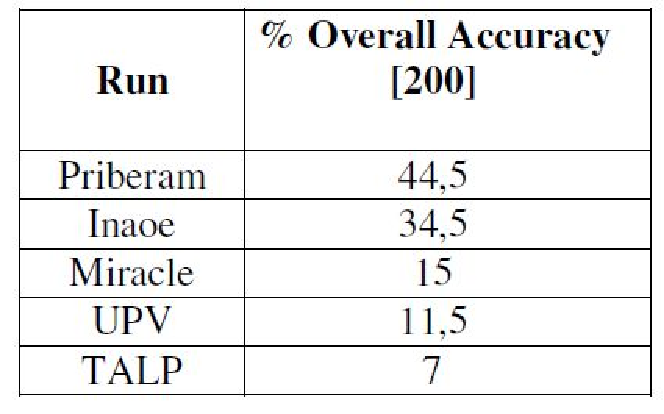
\includegraphics[scale=0.4]{graficos/resultados-espaniol-resumen}
    \caption{Competidores español}
  \end{figure}
\end{column}%
\hfill%
\begin{column}{.48\textwidth}

  \begin{figure}
      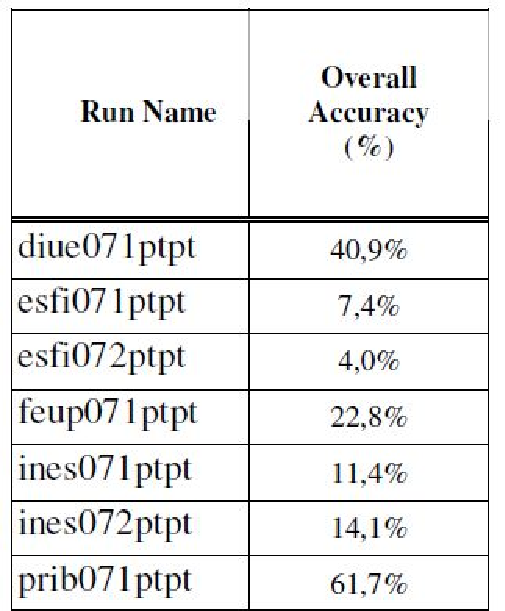
\includegraphics[scale=0.4]{graficos/resultados-portugues}
    \caption{Competidores portugués}
  \end{figure}
\end{column}%
\end{columns}

\end{frame}



\begin{frame}
\frametitle{Corrida 3: Respuestas ES}
\fontsize{7.5pt}{7.2}\selectfont
\begin{table}
\centering
\begin{center}
\begin{tabular}{|p {6cm} | l |}

Q & A\\ 
¿De dónde es típica la ensaimada? & Mallorca \\
¿De cuántos bits era este procesador? & 8 bits \\
¿En qué fecha El Corte Inglés compró Galerías Preciados? &  24 de noviembre de 1995\\
¿Qué empresa preside Steve Jobs? &  Apple Computer \\
¿Dé qué organización es comisionado David Stern? &  NBA\\
¿Qué animales tiran del carro de Cibeles? & leones\\
¿Cuántos Premios Goya ganó \dq{Torrente: El brazo tonto de la ley}? & dos\\
¿Quién fue la primera mujer que viajó al espacio? & Valentina Vladimírovna Tereshkova\\
¿A cuántos kilómetros de Huesca está el Castillo de Loarre? &   35 kilómetros\\
¿Cuál es el nombre del presidente de Burundi que murió en 1994? &  Cyprien Ntaryamira\\
¿Qué día se promulgó la constitución española de 1812?  & 19 de marzo\\
¿Qué dibujó Leonardo Da Vinci en 1492? & Hombre de Vitruvio\\
¿Qué programa de televisión presentó Takeshi Kitano de 1986 a 1989? &   Humor Amarillo\\
\end{tabular}
\caption{Respuestas español - $10.65\% = \frac{13}{122}$}
\end{center}
\end{table}
\end{frame}

\begin{frame}
\frametitle{Corrida 3: Respuestas PT y observaciones}

\begin{table}
\centering
\begin{center}
\begin{tabular}{| p {7cm} | l |}
Q & A\\ 
De que estado foi governador Adhemar de Barros? & São Paulo\\
Quando foi fundado o Nacional da Madeira? & 8 de Dezembro de 1910\\
\end{tabular}
\caption{Respuestas portugués - $1.92\% = \frac{2}{104}$}
\end{center}
\end{table}

Observaciones
\begin{itemize}
  \item Español peor que en 2.3 para muchas métricas
  \begin{itemize}
  \scriptsize{
      \item Español: 10.65\% exacto con una sola respuesta! 
      \item No es el peor
    }
  \end{itemize}
  \item Portugués: baja performance
  \begin{itemize}
  \scriptsize{
    \item Apenas un 3.16\% considerando la métrica $MRR_5$. 
    \item Las herramientas para portugués no son tan maduras como las herramientas para español; 
    \item Todo el desarrollo y el análisis estuvo basado en español (POC soporte otro idioma)
    }
  \end{itemize}

\end{itemize}

\end{frame}


\subsubsection*{Limitaciones, trabajo futuro, conclusiones}


\begin{frame}
\frametitle{Conclusiones: Dominio abierto}

Sobre modelo de dominio abierto:
  \begin{itemize}
 \item Impresión: falta de una \dq{doctrina} formal teórica accesible sobre generación de respuestas. ¿Oportunidad?
 \item Una mejora argumentada y con cierta presencia en la literatura del área fue el mecanismo de generación de queries que llamamos Lasso (por el sistema en el que fue implementado por primera vez) y nosotros lo incorporamos aquí, 
  \begin{itemize}
    \item  mejoras mínimas en la performance, de 7.75 a 7.81 en $MRR_1$ exacto (+0.26), de 8.94 a 9.27 en $MRR_5$ exacto (+0.31). 
  \end{itemize}
  \end{itemize}
Mejoras
 \begin{itemize}
  \item Módulo de \textit{focus} open source en inglés. Problema acotado, bien definido e inexistente. Herramienta útil.
  \item Módulo multilingüe de Question Classification.
  \item Mejorar las heurísticas
\end{itemize}

\end{frame}
